\chapter*{Published Research Paper 1}
\addcontentsline{toc}{chapter}{Published Research Paper 1}



	\section*{A Review on Smart Helmet}
\vspace{.3cm}

\begin{center}
	Gulshan Kumar Sharma, Raghav Kalra, Rishi Gaur, Roshni Kumari, Dr. Shikha Saxena
\\Department of Computer Science and Engineering
\\Krishna Engineering College, Mohan Nagar, Ghaziabad, Uttar Pradesh, India
\\ \{ gulshansharma011, raghavkalra3151, rishigaur12rg, sroshni24699, shikhasaxena83 \}   \\@gmail.com
\vspace{.3cm}
\end{center}
\textbf{Abstract:} Road accidents is one of biggest causes of deaths that exist in today’s scenario. The major causes of it comprises of drunk driving, rash driving and not to follow the traffic rules. In this paper, through a newly built system named “A Smart Helmet”, a solution to this problem has been suggested. The aim of this work is to suggest a user-friendly and low-cost protection system for the safety of the rider. Only when the rider is not- drunk and is wearing helmet, he will be able to ride his two-wheeler. The main purpose is to reduce the injuries happened to the rider during the accident and to provide immediate help and medical aid.
\vspace{.3cm}

\textbf{Keywords:} Road accidents, drunk driving, safety, healthcare, 2-wheeler helmet unit, helmet, vehicle unit.

\section*{1. INTRODUCTION}
Now, the road safety is the biggest cause of concern for the society. Drunk driving, rash driving and unwillingness to follow the traffic rules are the major causes of road accidents. A per the reports of the leading daily of September 2019, one death is being reported in every 4 minutes in India due to the road accidents. Not wearing the helmet is one of the major causes of two wheeler’s road accidents. In 2018 approximately 43600 riders died in road accident due to not wearing of the helmets. Drunk driving is another major concern of road accident.\vspace{.3cm}
 
In the present era, the invention of safety and smart helmets has become so important. With the technological development and better and powerful engines, the safety of the rider is of the top most concern. For 2-wheelers, helmet is the most important accessory of safety. But still a lot needs to be done in this area to provide a safe and the most comfortable travel to the riders of the two-wheeler.

\section*{2. RELATED WORK}
Researchers and engineers have proposed many designs for providing the safety system to the 2-wheeler riders. For the detection of a road accident, smart helmets with vibration sensors have been designed. But installation of the vibrating sensing devices in the internal area of the helmet is always not a good idea for detecting an accident as even the system can consider the accidental fall of the helmet to be an accident and unnecessarily send the notification.\vspace{.3cm}
 
Designing an accident alert system is very much required for providing immediate first-aid and medical help to the injured rider. Force sensing resistor {FSR} and BLDC Fan has been designed for detecting the riders head the motorcycle’s speed respectively. When the helmets strap is buckled the two-wheeler gets started. While riding wearing a wrist watch is not suggested. In this paper, a system named “A Smart Helmet” has been suggested.  It helps in the detection of the efficiency of the driver’s sobriety and its presence. The system is well managed and is user friendly.

\section*{3. METHODOLOGY}

“A Smart Helmet” has been made in order to save the rider. This Helmet is made in such a way that if any of the above 3 condition’s is met, the Vehicle will not start. The only purpose for making this Helmet System is to save as many lives during road accidents.\vspace{.3cm}

\begin{itemize}
	\item The following 3 conditions are:\vspace{.3cm}
	
	\begin{enumerate}
		\item 	Helmet is must to be worn by the rider,
		\item 	Strap of the Helmet must be Buckled
		\item 	Rider must be sober
	\end{enumerate}
	\item  All 3 conditions mentioned above are continuously monitored just to confirm, will the riding rules be followed or not.
	\item It comprises of smart accident detection system which helps in the detection of an accident.
	\item  It automatically sends the message in case of an accident to the given contact.
	\item  The System is easy to handle, user friendly and is very cheap.	
\end{itemize}

\begin{figure}[h]
	\centering
	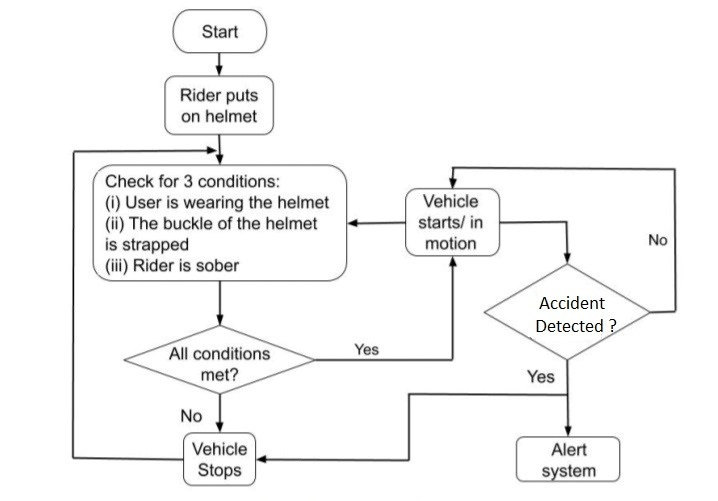
\includegraphics[scale=.55]{Flow diagram of the system.jpg}
	\captionsetup{labelformat=empty}
	\caption[]{Flow diagram of the proposed system.}
\end{figure}\vspace{.3cm}

After the rider put on the Helmet, only then the above 3 conditions are being checked. After their fulfilment, the Vehicle get start. After then, 3 parameters will gets monitored continuously. If any of the parameters are not met at any time, the Vehicle will get stop. All these functions are reached by dividing the System into 2 parts:

\begin{enumerate}
	\item 	Helmet Unit
	\item	Vehicle Unit
\end{enumerate}

Helmet and the Vehicle Units are connected with each other. Microcontroller is used for the system.\vspace{.3cm}

The Helmet Unit is kind of a transmitter circuit. It collects information required for the module to function from the number of sensors. The Vehicle Unit is dependent on the information received from the helmet. The functionality of the system is described below:

\section*{A. Helmet Unit}
The Helmet Unit is made up of various sensors which collect the required information from the surrounding and then process it to the microcontroller for processing.\vspace{.3cm}

It is rechargeable and battery-powered. Rechargeable battery supplies power to the whole circuit. The battery level indicates the available power and it indicates the rider when empty. USB type charging port is used to charge the battery.

\begin{figure}[h]
	\centering
	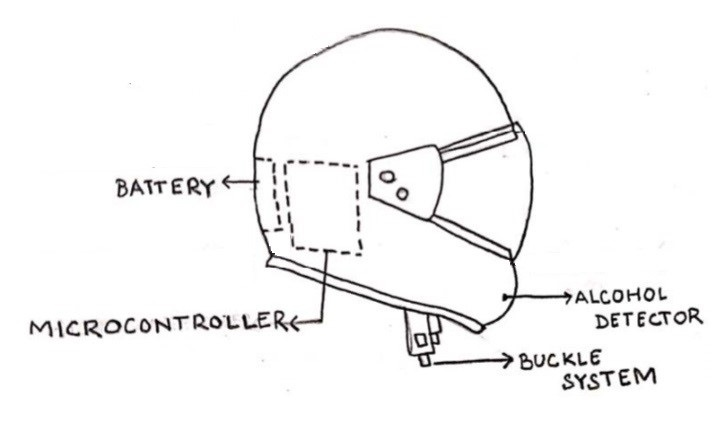
\includegraphics[scale=.5]{helmet unit.jpg}
	\captionsetup{labelformat=empty}
	\caption[]{Proposed Design Of The Helmet Unit.}
\end{figure}

The buckle is used as a security measure for the head of the rider in order to protect him from any accident. It uses a Single Pole Double Throw switch to provide enough security to the rider.\vspace{.3cm}

The Alcohol detector is a Gas Sensor for the detecting presence of alcohol (if any). An appropriate threshold value is set according to the laws of road safety.\vspace{.3cm}

The microcontroller section is where the microcontroller is placed. It is used for capturing the signals from the detectors. Data is processed and output is generated. This output is then sent to the vehicle unit for further functionality.\vspace{.3cm}

Then the analysis of combined outputs from all the subsystems and sensors is done. Depending on the three primary conditions which needs to be confirmed, the microcontroller then generates a Boolean value. That value is transmitted over to the Vehicle Unit.\vspace{.3cm}
\begin{figure}
	\centering
	\includegraphics[width=0.55\linewidth]{"images/working flow diagram"}
	\captionsetup{labelformat=empty}
	\caption[]{Flow diagram demonstrating the working of helmet unit.}
\end{figure}\vspace{.3cm}

\section*{i) Buckle System:}
\begin{itemize}

\item A buckle strap which is seen hanging from the head of the helmet. In case of an accident, if the buckle is not in place, the helmet might come off the rider’s head causing serious injuries to the rider.
\item	The buckle is kind of an automatic switch by which the transmission circuit in the helmet is turned on. This helps in saving power by keeping the transmission unit off, when it is not in use. It ensures that the vehicle’s ignition is not on unless the strap is buckled. If the strap is not buckled, then  there  is no  power  to  the  transmission system.
\item	A Single Pole Double Throw switch is used for achieving this functionality. The buckle system is diagrammatically demonstrated in below:

\end{itemize}
\begin{figure}[h]
	\centering
	\includegraphics[width=0.7\linewidth]{"images/buckle working"}
	\captionsetup{labelformat=empty}
	\caption[]{A simple diagram demonstrating working of buckle system.}	
\end{figure}

\section*{ii) Microcontroller System:}
Once the user buckled up the strap then transmission circuit which includes the microcontroller, is powered on. Then firstly the wireless communication with the Vehicle Unit is established. It further captures signals from the detectors.
\begin{itemize}
	\item a) Presence Detection: The presence detection system makes it clear that the vehicle is not going to start unless the rider is wearing the helmet. The system must be able to differentiate between a living and non- living object. The placement of the system is critical in order to eliminate any false alarms and to limit the sensor range. A PIR sensor used in this module actually generates a simple digital high or digital low value on detecting the human presence or not respectively. A buzzer, in the Vehicle Unit, buzzes a warning whenever the helmet is not worn by the rider.
	\item b) Alcohol Detection: Checking that the rider is sober or not is the third primary condition. The MQ-3 sensor is a gas sensor which checks for the alcohol content. When the rider’s breath falls on it, it tries to detect the presence of the alcohol in it above the threshold value which is set beforehand. It gives a Boolean False output if no alcohol is being detected and a True value if the alcohol is detected.
\end{itemize}
The placement of alcohol sensor is important as the driver’s breath should repeatedly fall on it for the detection purpose. If the rider is not drunk, the microcontroller receives a Boolean 1 from the alcohol sensor. Following this, the microcontroller then transmits a Boolean 0 value to the vehicle unit which stops the vehicle from starting. A buzzer blows again in order to signify non- sobriety of the driver.\vspace{.3cm}

The presence detection and sobriety detection are done simultaneously by the controller. If both the constrains are met, then Boolean 1 signal is sent to the Vehicle Unit in Boolean form from the controller in the Helmet Unit in order to start the vehicle.

\section*{iii) Battery:}
The system utilises a battery having max power requirement of Five Volt to start the transmission unit. The buckle works as a key between the power supply and the rest of the system. The transmission unit gathers to the point data and transmits it to the vehicle unit which performs the next suitable actions based on this data. The Vehicle Unit processes this data and takes suitable actions.
\section*{B. Vehicle Unit}
The Vehicle Unit is a part of the 2-wheeler. It is remotely paired to the Helmet Unit and it can be placed anywhere on the vehicle by selecting a position which is less prone to the accidents. The Vehicle Unit manages the ignition system of the vehicle. It is connected to the ignition system as shown in the figure. Nearly all vehicles work on two-wire or four-wire ignition key switches and the “Smart Helmet” System is suitable with both. 

\begin{figure}
	\centering
	\includegraphics[width=0.7\linewidth]{"images/Vehicle unit"}
	\captionsetup{labelformat=empty}
	\caption[]{Proposed design for the system to be installed on vehicle.}
\end{figure}

The Vehicle Unit is powered with the battery of the vehicle unit as it is rechargeable. The microcontroller is attached to the battery for the transmission of the power. This microcontroller accepts the signals from the microcontroller in the Helmet Unit and then it further processes the accepted data. The microcontroller and the ignition key switch are attached to each other through a relay module (one channel five Volt relay module) which generally controls the ignition of the vehicle which is based on the values accepted from the controller.\vspace{.3cm}

The Alert system includes an accident detection and a messaging system which in case of critical situations and accidents gets provoked. In case of the event of any mishappening, the GSM unit is used to generate an emergency message and send it to the emergency contact of the rider.\vspace{.3cm}

The buzzer blows to indicate an action or an warn in case of absence detection and alcohol detection system.

\begin{figure}[h]
	\centering
	\includegraphics[width=0.7\linewidth]{"images/vehicle unit working"}
	\captionsetup{labelformat=empty}
	\caption[]{Flow diagram demonstrating the working of vehicle unit.}
\end{figure}

\section*{Microcontroller System: }
This sub-part manages the most important functions of the Vehicle Unit. The reception unit accepts a value from the transmission unit and it then chooses on the actions to be taken afterwards. If the value accepted is 1 in Boolean, it means that all primary 3 constrains are met. On accepting 1 value from the Helmet Unit, the controller switches on the relay and the power is permitted to flow through the ignition system and then the vehicle ignites. If a Boolean 0 value is accepted, it means that some constrains from the 3 primary constrains are not satisfied. So, the switch of the relay remains tuned off and the vehicle doesn’t ignite. If at some point during the trip, the rider removes the helmet or some constrain goes to 0 then, the bike will automatically stop after giving a fair alert of 120 to 300 seconds. This is sufficient time for the driver for reaching a safer place and to stop the vehicle.

\section*{C. Communication Protocols}
As discussed above, the Helmet and the Bike System communicate with each other remotely. Since both the Helmet and the Bike Systems are not more than five hundred centimetres aside, a short-range wireless communication protocol can be used.\vspace{.3cm}

\textbf{Transceiver: }R-F Transmitter on Helmet Unit sends Signals to R-F Receiver on Vehicle Unit. As soon as R-F Transmitter gets power supply from Batteries, it will send Signals to R-F Receiver and fifth led on R-F Receiver will be on and finally, a Connection will be set up in between Helmet and Vehicle Unit.

\section*{4. RESULTS AND DISCUSSION}
\section*{A.	Smart Helmet System }
A good quality Helmet is used for this project. R-F Transmitter with Alcohol Detector System along with Batteries are fitted inside the Helmet.
\begin{figure}[h]
	\centering
	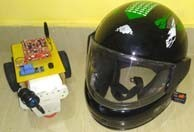
\includegraphics[width=0.7\linewidth]{images/dsfs}
	\captionsetup{labelformat=empty}
	\caption[]{“Smart Helmet” System.}
\end{figure}

\section*{B. Installation of Vehicle Unit on two-wheeler }
GSM System along with R-F Receiver has been fitted on Bike’s tank. 
\begin{figure}[h]
	\centering
	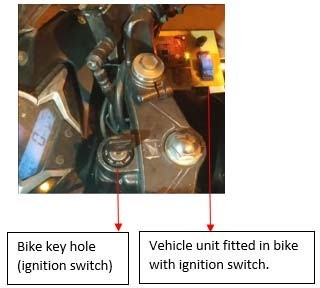
\includegraphics[width=0.7\linewidth]{images/bhjb}
	\captionsetup{labelformat=empty}
	\caption[]{Vehicle unit installed in bike.}
\end{figure}

\pagebreak
\section*{C. Presence and Alcohol detection in the system }
The serial monito r’s output is shown in Fig 9 shows that first the buckle system switches on the “Smart I met” System. Then, if the rider is wearing the helmet and he is sober, then the Hel met Unit detects. Depending on these values, it then sends a confirmation to the Vehicle Unit. This  action is performed several times in a loop till the system is on  .

\begin{figure}[h]
	\centering
	\includegraphics[width=0.7\linewidth]{"images/Status of rider"}
	\captionsetup{labelformat=empty}
	\caption[]{Status of Serial monitor when rider wears the helmet.}
	\label{fig:status-of-rider}
\end{figure}


The alcohol detection system determines the sobriety of the rider. When the helmet is worn, the alcohol sensor checks the breath of the individual.  As  shown  in  Fig 9,  if the value received from the sensor is ‘0’ then the ride is sober or vice versa.

\section*{D. Accident Detection System}
When a vehicle met with an accident, a message is being sent to the given emergency contact.
\begin{figure}
	\centering
	\includegraphics[width=0.7\linewidth]{"images/fas sa"}
	\captionsetup{labelformat=empty}
	\caption[]{Sent Message to Given Emergency Contact.}
	\label{fig:fas-sa}
\end{figure}



\section*{E. Power System of Vehicle Unit}
To control the Vehicle Unit, prototype a 9V rechargeable battery is used.
\begin{figure}
	\centering
	\includegraphics[width=0.4\linewidth]{"images/faf af"}
	\captionsetup{labelformat=empty}
	\caption[]{Vehicle unit with rechargeable battery}
	\label{fig:faf-af}
\end{figure}


\section*{5. CONCLUSION}
“A Smart Helmet” System can be considered as a magnificent system in order to bear safety to the drivers of the 2-wheelers. The system doesn’t allow the driver to drive his/her bike without wearing his/her helmet. The driver can only drive his/her vehicle when he/she is not drunk and has strapped his/her helmet. The system is very user-friendly and easy to use.\vspace{.3cm}

As future implementation a system that uses power straight away from the vehicle or flexible solar panels can be used for well-planned usage of the power. A mobile sensor that doesn’t allow the driver from using his/her phone while driving his/her vehicle can be used for secure travel. A camera can be mounted to record the emergencies and accidents when SOS key is pressed. On the event of failure of system of any kind, a back-up alternative in the form of a mobile application can be provided.  \vspace{.3cm}

Pricing policies play the most exclusive role in the development of the item and makes business practice more stable and natural. Eventually, the Smart Helmet will put a figure around Rs.5500-6500/- including microcontrollers, sensors, transportation, and work cost. It can be further reduced by 40\% with mass production.


\section*{REFERENCES}

[1] R. Vashisth, S. Gupta, A. Jain, S. Gupta, Sahil and P. Rana, "Implementation and analysis of smart helmet," 2017 4th International Conference on Signal Processing, Computing and Control (ISPCC), Solan, India, 2017, pp. 111-117, doi: 10.1109/ISPCC.2017.8269660.\\ 
$[2]$ International Journal of Science and Research (IJSR) ISSN (Online): 23197064 Volume 3 Issue 3, March 2014 \\
$[3]$ J. International Journal Of Computer Science And Applications Vol. 6, No.2, ISSN: 0974-1011, Apr 2013 \\
$[4]$ Sayeed and A.Perrig, Secure Wireless Communications: Secret Keys through Multi-path,Proc.IEEE Intl Conf.Acoustics, Speech Signal Processing, pp. 3013-3016, Apr.2008 \\
$[5]$ International Journal of Scientific Engineering Research Volume 2, Issue 12, 1 ISSN 2229-5518 , December-2011 \\
$[6]$ Drunken driving protection system International Journal of Scientific Engineering Research Volume 2, Issue 12, 1 ISSN 2229-5518, December2011.\\
$[7]$ Aagaahi - A Smart Helmet (Date Added to IEEE Xplore: 16 September 2020) \\

\chapter*{Remarks}
\addcontentsline{toc}{chapter}{Remarks}

This research paper is published in IJARESM,  February 2021 issue.


\vspace{.3cm}

\begin{flushleft}
	You can view or download published research paper from link below $\downarrow$\\
\end{flushleft}
http://www.bit.ly/36xcdoE
